\documentclass[reprint,english,notitlepage]{revtex4-1}  % defines the basic parameters of the document

% if you want a single-column, remove reprint

% allows special characters (including æøå)
\usepackage[utf8]{inputenc}
\usepackage[english]{babel}
\usepackage{parskip}

%% note that you may need to download some of these packages manually, it depends on your setup.
%% I recommend downloading TeXMaker, because it includes a large library of the most common packages.

\usepackage{physics,amssymb}  % mathematical symbols (physics imports amsmath)
\include{amsmath}
\usepackage{graphicx}         % include graphics such as plots
\usepackage{xcolor}           % set colors
\usepackage{hyperref}         % automagic cross-referencing (this is GODLIKE)
\usepackage{listings}         % display code
\usepackage{tikz}             % draw figures manually
\usepackage{listings}         % display code
\usepackage{subfigure}        % imports a lot of cool and useful figure commands
%%\usepackage{float}
\usepackage{nicematrix}
\usetikzlibrary{quantikz}
%\usepackage[section]{placeins}
\usepackage{algorithm}
\usepackage[noend]{algpseudocode}
\usepackage[style=numeric,backend=bibtex,sorting=none]{biblatex}
\addbibresource{sources1.bib}

% defines the color of hyperref objects
% Blending two colors:  blue!80!black  =  80% blue and 20% black
\hypersetup{ % this is just my personal choice, feel free to change things
    colorlinks,
    linkcolor={red!50!black},
    citecolor={blue!50!black},
    urlcolor={blue!80!black}}

%% Defines the style of the programming listing
%% This is actually my personal template, go ahead and change stuff if you want
\lstset{ %
	inputpath=,
	backgroundcolor=\color{white!88!black},
	basicstyle={\ttfamily\scriptsize},
	commentstyle=\color{magenta},
	language=Python,
	morekeywords={True,False},
	tabsize=4,
	stringstyle=\color{green!55!black},
	frame=single,
	keywordstyle=\color{blue},
	showstringspaces=false,
	columns=fullflexible,
	keepspaces=true}


%% CREATING THE .pdf FILE USING LINUX IN THE TERMINAL
%% 
%% [terminal]$ pdflatex template.tex
%%
%% Run the command twice, always.
%% If you want to use \footnote, you need to run these commands (IN THIS SPECIFIC ORDER)
%% 
%% [terminal]$ pdflatex template.tex
%% [terminal]$ bibtex template
%% [terminal]$ pdflatex template.tex
%% [terminal]$ pdflatex template.tex
%%
%% Don't ask me why, I don't know.

% Deadline October 7 
\begin{document}
\title{Project 1 on Machine Learning}   % self-explanatory
\author{Oskar Hafstad, Simon H. Hille \& Semya A. Tønnessen}               % self-explanatory
\date{\today}                             % self-explanatory
\noaffiliation                            % ignore this
\begin{abstract}                          % marks the beginning of the abstract
Github repo for this paper: \url{https://github.com/hafos/FYS-STK4155}
\vspace{3mm}

The aim of this project is to study linear regression methods by fitting a two dimensional polynomial onto two different datasets. 
%In this project the aim is to study three different regression methods for approximating a 2D dataset. 
Using Ordinary Least Squares (OLS), Ridge regression and Lasso regression, we attempt to estimate the best fit for the two dimensional function called Franke's function and then for real topographic data. 
% We also study the effect of adding noise to the Franke function. 
The model is optimized by performing bootstrap resampling and (5-10)-fold cross validation resampling techniques, and we perform an error analysis by studying the Mean Square Error (MSE) and bias-variance trade-off. 

% Also present results with error margins 
For the Franke function
%, calculated for a $XX\times XX$ grid, 
we find an optimal model for OLS regression with a polynomial degree $X = X$. Meanwhile, for the Ridge regression we find both the optimal polynomial, $X = X$, and the optimal penalty parameter, $\lambda^\text{Ridge} = XXX$, for a $d\cross\lambda$ grid. For the Lasso regression we find the optimal fit for $X = X$ and $\lambda = XXX$. 
The MSE score found when using Ridge regression and Lasso regression were not notably smaller than the score we found when using the OLS method, and so the OLS regression method is a good fit for the Franke function. 
The analysis is repeated for the terrain data, consisting of a part of the Tin Bider crater located in the Sahara desert. 
The best fit using OLS was found for $ X = X$. For Ridge, the best model was for $ X = X$ and $\lambda^\text{Ridge} = X$. 
Lasso might be quite computationally expensive, particularly for small $\lambda$, and should not yield much better results than Ridge. We therefore conclude that the Ridge model finds the best fit. 
\end{abstract}                            % marks the end of the abstract
\maketitle                                % creates the title, author, date & abstract

%\autocite{quantum_hist}

%__________________________________________________________________________

\tableofcontents

\section{Introduction} 

% It is vital to properly communicate precisely what has been done, what the results are and their implications. The motivation for this is to make the work understood and reproducible, so that others can both check and build on your work.

% The main purpose of the introduction section is to provide context and motivation for the work. It is also common --- and quite useful --- to use the last paragraph of the introduction to outline the rest of the report, to tell the reader what they should expect in the different sections.

% Motivate what we do 
In this report we familiarize ourselves with analysis of linear regression methods, which are methods that attempt to model the relationship between variables by fitting a linear equation to observed data. Linear regression models can be quite useful, as they are simple and often provide an adequate description of how input affects nonlinear models, particularly when using small numbers of training cases, low signal-to-noise ratio or sparse data. 

We will attempt to fit three predictive models, using the methods Ordinary Least Squares (OLS), Ridge regression, and Lasso regression, to two datasets. The first dataset is a $XX \times XX$ grid with values computed using the two-dimensional Franke function, for which we add normally distributed noise $N(0,\sigma^2)$. This function is  widely used when testing various interpolation and fitting algorithms. The other dataset consists of terrain based on real topographic data from the Tin Bider Crater located in the Sahara desert in Algeria. 

The optimal set of parameters $\boldsymbol{\hat{\beta}}$ will be determined by fitting a two-dimensional polynomial onto the datasets and minimizing the error. 
After establishing the model and the method, we employ resampling techniques such as cross-validation and bootstrap, in order to optimize the models and test their validity. We also study the Bias-Variance trade-off in an attempt to find for which polynomials $XXX$ and penalty parameter $\lambda$ we find the best fit for the different models. For Ridge and Lasso regression we expect to see that we can compute more complex models, as these reduce the chance for overfitting. However, the methods are more computationally heavy, and we therefore need to determine the best model depending on the dataset we model. 

In section \ref{sec:methods} we provide an overview of OLS, Ridge regression, and Lasso regression, in addition to presenting the datasets and noise, including a description of how we set up the model and design matrix and how we split and scale the data. We also present various methods of evaluating the accuracy of each method. A selection of results relevant to our understanding are presented in section \ref{sec:results}. In section \ref{sec:discussion} we discuss how our results correspond to our expectations, and in section \ref{sec:conclusion} we provide a short summary and outlook. 


%\section{Theory}                    % (optional) 
%_______________________________METHOD___________________________________________
\section{Method}\label{sec:methods}

% Part a) 
We assume the existence of a continuous function $f(\boldsymbol{x})$ and a normal distributed error $\boldsymbol{\varepsilon} \sim N{\left( 0, \sigma^2\right)}$ which describes our data 
\begin{align}\label{eq: model}
    \boldsymbol{y} = f(\boldsymbol{x}) + \boldsymbol{\varepsilon}, 
\end{align}
where $\boldsymbol{y}\in\mathbb{R}^n$ consists of $n$ observed values $y_i$.  
We want to use linear regression to approximate the function $f(\boldsymbol{x})$ with a model $\boldsymbol{\tilde{y}}$. 
There are many different techniques for such calculations, and we will study three of these; one using least squares estimation, and two using penalised estimation. 
% Observed values \boldsymbol{y} 
% Approximate values \boldsymbol{\tilde{y}} predicts the true value 

The function $f$ is approximated by $\boldsymbol{\tilde{y}}$, 
\begin{align}\label{eq: y_approx}
    \boldsymbol{\tilde{y}} = \boldsymbol{X}\boldsymbol{\beta}, 
\end{align}
where the matrix $\boldsymbol{X}\in\mathbb{R}^{n\times p}$ is the design matrix, containing $n$ rows with vectors $\boldsymbol{x}_i\in\mathbb{R}^p$, and $\mathbf{\beta}\in\mathbb{R}^p$ are the unknown parameters we want to determine. 

% Find the expectation value of the model y for a given element i and its variance 
For an observed value $y_i$, 
\begin{align}
    y_i &= \sum\limits_{j=0} x_{ij}\beta_j + \varepsilon_j %\nonumber \\ 
        = \boldsymbol{x}_{i,*}\boldsymbol{\beta} + \varepsilon_j, 
\end{align}
where $*$ means that we iterate over the whole column. The product $\boldsymbol{x}_{i,*}\boldsymbol{\beta}$ is non-stochastic, meaning it is deterministic and therefore $\mathbb{E}[\boldsymbol{x}_{i,*}\boldsymbol{\beta}] = \boldsymbol{x}_{i,*}\boldsymbol{\beta}$. Per definition, $\sigma\sim N(0,\sigma^2)$ is normalized, thereby making $\mathbb{E}[\varepsilon_i] = 0$. 

We thus find that the expectation value of $\boldsymbol{y}$ for a given element $i$ is 
\begin{align}
    \mathbb{E}[y_i] 
    & = \mathbb{E}[\boldsymbol{x}_{i,*}\boldsymbol{\beta} + \mathbb{E}\varepsilon_i] \nonumber \\ 
    & = \mathbb{E}[\boldsymbol{x}_{i,*}\boldsymbol{\beta}] + \mathbb{E}[\varepsilon_i] \nonumber \\ 
    & = \boldsymbol{x}_{i,*}\boldsymbol{\beta}. 
\end{align}

The variance of this variable is 
% found from the expectation value of the outer product $\boldsymbol{yy}^T$ XXX ? 
% E[yy^T] ??? 
\begin{align}
    \text{Var}[y_i] 
    & = \nonumber \\ 
    & = \sigma^2. 
\end{align}

Hence, $y_i\sim N(\mathbf{X}_{i,*}\boldsymbol{\beta}, \sigma^2)$, that is $\boldsymbol{y}$ follows a normal distribution with mean value $\mathbf{X}\boldsymbol{\beta}$ and variance $\sigma^2$. 

We may obtain the optimal estimation, $\hat{\mathbf{\beta}}$, of $\mathbf{\beta}$ by minimizing the cost function $C(\boldsymbol{X}, \mathbf{\beta})$. 
The cost function measures by how much our model deviates from the observed values, and from it we obtain $\mathbf{\beta}$. 






\subsection*{Error Analysis}
We can predict the error by looking at the Mean Square Error, which is the mean value of the square of the errors between approximations and the measured values, 
\begin{align}\label{eq: MSE}
    MSE\left(\boldsymbol{y},\boldsymbol{\tilde{y}}\right) = \frac{1}{n}\sum\limits_{i=0}^{n-1}{\left(y_i - \tilde{y}_i\right)}^2
\end{align}
as well as evaluating the $R^2$ score function, 
\begin{align}\label{eq: R2}
    R^2 \left(\boldsymbol{y},\boldsymbol{\tilde{y}}\right) = 1 - \frac
    {\sum\limits_{i=0}^{n-1}{y_i - \tilde{y}_i}^2}
    {\sum\limits_{i=0}^{n-1}{y_i - \bar{y}_i}^2}
\end{align}
where we define the mean value of $\boldsymbol{y}$ as 
\begin{align}\label{eq: mean_y}
    \bar{y} = \frac{1}{n}\sum_{i=0}^{n-1} y_i. 
\end{align}


%-----------------------------------Bias-Variance trade-off-----------------------------------
\subsubsection*{Bias-variance trade-off}
% Part c) Bias-variance trade-off and resampling techniques 
When we have obtained $\boldsymbol{\beta}$, we need an estimate of how good our approximation is. We will therefore also study the bias-variance trade-off in the context of continuous predictions such as regression. 

In order to find a measure of the expected error in our function we optimize the means squared error via the cost function, 
\begin{align}\label{eq: Cost Function}
    C(X, \boldsymbol{\beta}) = \frac{1}{n}(y_i - \tilde{y_i})^2 = \mathbb{E}\left[(\boldsymbol{y}  -\boldsymbol{\tilde{y}})^2\right]. 
\end{align}

Here the expected value $\mathbb{E}$ is the sample value. 
We can rewrite this in terms of a term which contains the variance of the model itself. This variance term measures the deviation from the true data and the mean value of the model, called the bias term, and finally the variance of the noise. 

We insert $\boldsymbol{y}$ for a model $\boldsymbol{y} = f(\boldsymbol{x) + \boldsymbol{\varepsilon}}$ into equation~\ref{eq: Cost Function}, 
\begin{align*}
    %C(X, \boldsymbol{\beta})
    \mathbb{E}[(\boldsymbol{y} - \boldsymbol{\tilde{y}})^2] 
    & = \mathbb{E}[(\boldsymbol{f} + \boldsymbol{\varepsilon} - \boldsymbol{\tilde{y}})^2] \\ 
    & = \mathbb{E}[\boldsymbol{\varepsilon}^2 + 2\boldsymbol{\varepsilon}(\boldsymbol{f} - \boldsymbol{\tilde{y}}) + (\boldsymbol{f} - \boldsymbol{\tilde{y}})^2] \\ 
    & = \boldsymbol{\sigma}^2 + \mathbb{E}[(\boldsymbol{f} - \boldsymbol{\tilde{y}})^2], 
\end{align*}
where $\boldsymbol{\sigma}^2$ is the error arising due to stochastic noise. 
We rewrite $\mathbb{E}[(\boldsymbol{f} - \boldsymbol{\tilde{y}})^2]$ by adding and subtracting $\mathbb{E}[\boldsymbol{\tilde{y}}]$, 
\begin{align*}
    \mathbb{E}[\boldsymbol{f} - \boldsymbol{\tilde{y}})^2] 
    & = \mathbb{E}[\boldsymbol{f} - \boldsymbol{\tilde{y}} + \mathbb{E}[\boldsymbol{\tilde{y}}] - \mathbb{E}[\boldsymbol{\tilde{y}}])^2] \\ 
    & = \mathbb{E}[(\boldsymbol{f} - \mathbb{E}[\boldsymbol{\tilde{y}}])^2 
        + (\mathbb{E}[\boldsymbol{\tilde{y}}] - \boldsymbol{\tilde{y}})^2] \\
        &+ \mathbb{E}[2(\boldsymbol{f} - \mathbb{E}[\boldsymbol{\tilde{y}}])
            (\mathbb{E}[\boldsymbol{\tilde{y}}] - \boldsymbol{\tilde{y}})] \\ 
    & = (\boldsymbol{f} - \mathbb{E}[\boldsymbol{\tilde{y}}])^2 
        + \mathbb{E}[(\boldsymbol{\tilde{y}} - \mathbb{E}[\boldsymbol{\tilde{y}}])^2]
\end{align*}

where $\mathbb{E}[\mathbb{E}[\boldsymbol{\tilde{y}}] - \boldsymbol{\tilde{y}}] = 0$ and $\mathbb{E}[(\boldsymbol{f} - \mathbb{E}[\boldsymbol{\tilde{y}}])^2] = (\boldsymbol{f} - \mathbb{E}[\boldsymbol{\tilde{y}}])^2$. 

Inserting into the cost function for the model yields: 
\begin{align}
    \mathbb{E}[(\boldsymbol{y} - \boldsymbol{\tilde{y}})^2] 
    &= (\boldsymbol{f} - \mathbb{\boldsymbol{\tilde{y}}})^2 
        + \mathbb{E}[\boldsymbol{\tilde{y}} 
        - \mathbb{E}[\boldsymbol{\tilde{y}}]] 
        + \boldsymbol{\sigma}^2 \nonumber \\ 
    &= (\text{Bias}[\tilde{y}])^2 
        + \text{Var}[\tilde{f}] 
        + \sigma^2, 
\end{align}

%The bias of the model $\boldsymbol{\tilde{y}}$ compared to the continuous function $\boldsymbol{f}$ that we wish to obtain is given by 
with 
\begin{align}
    (\text{Bias}[\tilde{y}])^2 = (\boldsymbol{y} - \mathbb{E}[\boldsymbol{\tilde{y}}])^2, 
\end{align}

and 

\begin{align}
    \text{Var}[\tilde{f}] = \frac{1}{n}\sum\limits_i (\tilde{y}_i - \mathbb{E}[\boldsymbol{\tilde{y}}])^2. 
\end{align}

A model having a high bias means that it predicts inaccurate results, even if we only see a small variance in these predictions. 
For a lower bias, with a higher variance, we have predictions that are centered around the true value, but vary quite a bit. 
When predicting the model we want to ensure the optimal bias-variance trade-off, in order to get the most trustworthy results. 

















%--------------------------------------------OLS--------------------------------------------
\subsection*{Ordinary Least Squares}
For the OLS method, we assume a cost function 
\begin{align}\label{eq: costfunc_OLS}
    C_\text{OLS}(\boldsymbol{\beta}) = \frac{1}{n}\left\{(\boldsymbol{y} - \mathbf{X}\boldsymbol{\beta})^T (\boldsymbol{y} - \mathbf{X}\boldsymbol{\beta})\right\},
\end{align}
which, when minimized, yields the OLS expression for the optimal parameter, 
\begin{align}\label{eq: optimal_OLS}
    \boldsymbol{\hat{\beta}}_\text{OLS} 
    = (\mathbf{X}^T \mathbf{X})^{-1} \mathbf{X}^T\boldsymbol{y} 
    = H^{-1} \mathbf{X}^T\boldsymbol{y} , 
\end{align}
where $H = \mathbf{X}^T \mathbf{X}$ is the Hessian matrix. We can solve this numerically using matrix inversion, if the matrix $\mathbf{X}^T \mathbf{X}$ is invertible. 

NOTE: We invert using pinv (psudoinvers) which inverts a matrix that is singular or near singular 
Our matrix $\mathbf{X}^T\mathbf{X}$ is a square matrix, ?, but it may be singular. The psudoinverse is the generalization of the matrix inverse for square matrices to rectangular matrices where the number of rows and columns are not equal. 


% Part a) With the OLS expressions for the optimal parameters beta-hat, show that the expectation value of beta-hat is beta 
With the OLS expression for the optimal parameter $\boldsymbol{\hat{\beta}}_\text{OLS} = \boldsymbol{\hat{\beta}}$, we can find the expectation value of this parameter, 
\begin{align}
    \mathbb{E}(\boldsymbol{\hat{\beta}}) 
    &= \mathbb{E}[(\mathbf{X}^{\top} \mathbf{X})^{-1}\mathbf{X}^{\top} \mathbf{Y}] \nonumber \\ 
    &= \mathbb{E}[(\mathbf{X}^{\top} \mathbf{X})^{-1}\mathbf{X}^{\top} (\mathbf{X}\boldsymbol{\beta} + \boldsymbol{\varepsilon})] \nonumber \\ 
    &= (\mathbf{X}^{\top} \mathbf{X})^{-1}\mathbf{X}^{\top} (\mathbb{E}[\mathbf{X}\boldsymbol{\beta}] + \mathbb{E}[\boldsymbol{\varepsilon}]) \nonumber \\ 
    &= (\mathbf{X}^{T} \mathbf{X})^{-1} \mathbf{X}^{T}\mathbf{X}\boldsymbol{\beta} \nonumber \\ 
    &=\boldsymbol{\beta}, \nonumber
\end{align}

where we have that $(\mathbf{X}^{T} \mathbf{X})^{-1} \mathbf{X}^{T}\mathbf{X}$ is the identity matrix. 

% Part a) Derive the variance of beta 
The variance is 
\begin{align}
    \text{Var}[\boldsymbol{\hat{\beta}}] 
    & = \mathbb{E} [ (\boldsymbol{\beta} 
        - \mathbb{E}[\boldsymbol{\beta}]) (\boldsymbol{\beta} 
        - \mathbb{E}[\boldsymbol{\beta}])^{T} ] \nonumber \\
    & = \mathbb{E} \{ [(\mathbf{X}^{T} \mathbf{X})^{-1} \, \mathbf{X}^{T} \mathbf{Y} 
        - \boldsymbol{\beta}] \, [(\mathbf{X}^{T} \mathbf{X})^{-1} \, \mathbf{X}^{T} \mathbf{Y} 
        - \boldsymbol{\beta}]^{T} \} \nonumber \\
    & = (\mathbf{X}^{T} \mathbf{X})^{-1} \, \mathbf{X}^{T} \, \mathbb{E} [\mathbf{Y} \, \mathbf{Y}^{T}] \, \mathbf{X} \, (\mathbf{X}^{T} \mathbf{X})^{-1} 
        - \boldsymbol{\beta} \, \boldsymbol{\beta}^{T} \nonumber \\
    & = (\mathbf{X}^{T} \mathbf{X})^{-1} \, \mathbf{X}^{T} \, \{ \mathbf{X} \, \boldsymbol{\beta} \, \boldsymbol{\beta}^{T} \,  \mathbf{X}^{T} 
        + \sigma^2 \} \, \mathbf{X} \, (\mathbf{X}^{T} \mathbf{X})^{-1} - \boldsymbol{\beta} \, \boldsymbol{\beta}^{T} \nonumber \\ 
    & = \boldsymbol{\beta} \, \boldsymbol{\beta}^{T} 
        + \sigma^2 \, (\mathbf{X}^{T} \mathbf{X})^{-1} 
        - \boldsymbol{\beta} \, \boldsymbol{\beta}^{T} \nonumber \\ 
    & = \sigma^2 \, (\mathbf{X}^{T} \mathbf{X})^{-1}, \nonumber 
\end{align}

where we use that $\mathbb{E}(\mathbf{YY}^{\top} = \mathbf{X}\boldsymbol{\beta\beta}^{\top}\mathbf{X}^{\top} + \sigma^2\mathbf{I}_{nn}$. We can use this expression to define a confidence interval for the parameters $\beta$. A given parameter $\beta_j$ is given by the diagonal matrix element of the above matrix. 




%--------------------------------------Ridge Regression--------------------------------------
\subsection*{Ridge Regression} 
The next method we want to analyze is Ridge regression, a method of estimating the coefficients of multiple-regression models in scenarios where the independent variables are highly correlated, which was developed as a possible solution to the imprecision of least square estimators when linear regression models have highly correlated independent variables. This should provide a more precise ridge parameter estimate, as its variance and mean square estimator are often smaller than other mean square estimators. However, this comes at the cost of computational time. 

We define the new cost function to be optimized by adding a penalty term, $\lambda||\beta||_2^2$ to equation~\ref{eq: costfunc_OLS}, where $\lambda\in\mathbb{R}$ is some value such that $\lambda > 0$: 
\begin{align}\label{eq: costfunc_ridge}
    C(\mathbf{X},\boldsymbol{\beta})_\text{Ridge} = \left\{ (\boldsymbol{y} - \mathbf{X}\boldsymbol{\beta})^T (\boldsymbol{y} - \mathbf{X}\boldsymbol{\beta}) \right\} + \lambda\boldsymbol{\beta}^T\boldsymbol{\beta}
\end{align}

By taking the derivatives with respect to $\boldsymbol{\beta}$ we find a modified matrix inversion problem for which finite values of $\lambda$ does not suffer from singularity problems. 
We thus obtain the optimal parameters 
\begin{align}\label{eq: optimal_ridge
}
    \boldsymbol{\hat{\beta}}_\text{Ridge} = {(\mathbf{X}^T\mathbf{X} + \lambda\mathbf{I})}^{-1} \mathbf{X}^T\boldsymbol{y}, 
\end{align}

where $\mathbf{I}$ is a $p\times p$ identity matrix where $\sum_{i=0}^{p-1}\beta_i^2\leq t$, where $t$ is a finite positive number. 

We should see that for specific values of $\lambda$, we may reduce the variance of the optimal parameters using Ridge regression, which will affect the bias-variance. 


%--------------------------------------Lasso Regression --------------------------------------
\subsection*{Lasso Regression}
We once more redefine the cost function, adding a penalty term $\lambda||\boldsymbol{\beta}||_1$ such that we obtain the cost function: 
\begin{align}\label{eq: costfunc_lasso}
    C(\mathbf{X},\boldsymbol{\beta})_\text{Lasso} 
    = \left\{ (\boldsymbol{y} - \mathbf{X}\boldsymbol{\beta})^T (\boldsymbol{y} - \mathbf{X}\boldsymbol{\beta}) \right\} + \lambda||\boldsymbol{\beta}||_1, 
\end{align}
for which we find, by taking the derivative with respect to $\boldsymbol{\beta}$, 
\begin{align}\label{eq: optimal_lasso}
    \mathbf{X}^T\mathbf{X}\boldsymbol{\beta} + \lambda sgn(\boldsymbol{\beta}) = 2\mathbf{X}^T\boldsymbol{y}, 
\end{align}
This equation can be solved by using standard convex optimization algorithms~\cite{morthen}, however performing the calculations is not trivial. We perform the analysis using the functionalities of `scikit-learn` in python. XXX



%---------------------------------------Error Analysis ---------------------------------------

\subsection{Resampling}
% we are looking for expectation values and an estimate of how accurate they are, i.e., possible sources for errors.
There is often some limit to the amount of data we may obtain, and therefore it can be vital to have methods for resampling this data in order to test it for large samples. Resampling approaches can be computationally expensive, as these involve fitting the same statistical method multiple times using different subsets of the training data. However, due to advances in computing power, this is not always an issue and for certain datasets it may improve the model considerably~\cite{morthen}. We consider two of the most commonly used resampling methods, the bootstrap and cross-validation. These can be used to study the validity of the optimal parameters $\boldsymbol{\hat{\beta}}$, which we obtain using either OLS, Ridge or Lasso regression. 

\subsubsection{Bootstrap resampling}
The bootstrap is widely used, as it is quite general. 
% Does not require distributional assumptions -> It can provide more accurate inferences when the data are not well behaved or when the sample size is small 
% Possible to apply the bootstrap to statistics with sampling distributions that are difficult to derive, even asymptotically 
% Relatively simple to apply the bootstrap to complex data-collection plans 
It is a non-parametric approach to statistical inference that substitutes computation for more traditional distributional assumptions and asymptotic results. 

We assume that we have some data $\boldsymbol{y}$ from which we estimate $\boldsymbol{\hat{\beta}}$, where $\boldsymbol{\beta}$ has a unknown probability distribution and thus it can be thought of as a random variable where $\boldsymbol{\beta}$ has the highest probability of being $\boldsymbol{\hat{\beta}}$. 

We may then draw with replacement $n$ numbers from the data $\boldsymbol{y} = (y_1, y_2, ..., y_n)$. Next we define a vector $\boldsymbol{y^*}$ containing the values which were drawn from $\boldsymbol{y}$, from which we can compute $\boldsymbol{\hat{\beta}}^*$ by evaluating $\boldsymbol{\hat{\beta}}$ under the observations $\boldsymbol{y}^*$. Repeating the process $k$ times yields a list of vectors. 
The relative frequency of the vectors $\boldsymbol{\beta}^*$ is the approximation of $p(\boldsymbol{\beta})$. 

XXX
When you are done, you can draw a histogram of the relative frequency of $\boldsymbol{\hat{\beta}}^*$. This is your estimate of the probability distribution p(t). Using this probability distribution you can estimate any statistics thereof. In principle you never draw the histogram of the relative frequency of $\boldsymbol{\hat{\beta}}^*$. Instead you use the estimators corresponding to the statistic of interest. For example, if you are interested in estimating the variance of $\boldsymbol{\hat{\beta}}$, apply the estimator $\sigma^2$ to the values $\boldsymbol{\hat{\beta}}^*$
XXX 

\subsubsection{Cross validation}
Cross-validation can be used to estimate the test error associated with a given statistical learning method in order to evaluate its performance, or to select the appropriate level of flexibility~\cite{morthen}. 
%he process of evaluating a model’s performance is known as model assessment, whereas the process of selecting the proper level of flexibility for a model is known as model selection. 


\subsection{Datasets}
In order to study the different regression methods, we must obtain datasets on which we can perform the analysis. 

% Test 
Before we begin the regression analysis on proper datasets, we implement a test where the design matrix $\mathbf{X}$ is set equal to the identity matrix 
\begin{align}\label{eq: identity_matrix}
    \mathbf{I} = 
    \begin{bmatrix} 
    1 & 0 & ... & 0 \\ 
    0 & 1 & ... & 0 \\ 
    : & : &     & : \\ 
    0 & 0 & ... & 1 
    \end{bmatrix}
\end{align}
and we assert that the mean square error is exactly equal to zero. % XXX actually do this 

% Franke function 
The first dataset we will use is called the Franke function, which is a weighted sum of four exponentials given as, 
\begin{align}\label{eq: frankie}
    f(x,y) = \frac{3}{4} \exp\left(
             -\frac{{\left( 9x-2\right)}^2}{4}
             -\frac{{\left( 9y-2\right)}^2}{4}
             \right) 
             \\ 
            +\frac{3}{4} \exp\left(
             -\frac{{\left( 9x+1\right)}^2}{49}
             -\frac{{\left( 9y+1\right)}}{10}
             \right) \nonumber
             \\ 
            +\frac{1}{2} \exp\left(
             -\frac{{\left( 9x-7\right)}^2}{4}
             -\frac{{\left( 9y-3\right)}^2}{4}
             \right) \nonumber
             \\ 
            -\frac{1}{5} \exp\left(
            -{\left(9x-4\right)}^2 - {\left(9y-7\right)}^2
             \right), \nonumber
\end{align}
defined for $x,y\in [0,1]$. 

We generate a dataset using $N$ uniformly distributed values of $x,y\in[0,1]$, adding some normally distributed noise $\epsilon = N(0, \sigma^2)$. The function which describes our data becomes 
\begin{align}
    \boldsymbol{y} = f(x,y) + N(0, \sigma^2). 
\end{align}
The model for this data, $\boldsymbol{\tilde{y}}$, can be obtained using the method described in section~\ref{sec:methods}. The Franke function is visualized without noise in figure~\ref{fig: ff}, and with noise $\sigma = XXX$ in figure~\ref{fig: ffn}. Both figures are plotted for uniformly distributed $x$ and $y$, on a $XXX \times XXX$ grid. 

\begin{figure}[h!]
    \centering %Centers the figure
    \includegraphics[width=1.0\linewidth]{Project 1/images/frankefunc.PNG} %Imports the figure.
    \caption{The Franke function }
    \label{fig: ff}
\end{figure}
\begin{figure}[h!]
    \centering %Centers the figure
    \includegraphics[width=1.0\linewidth]{Project 1/images/frankefuncnoise.PNG} %Imports the figure.
    \caption{}
    \label{fig: ffn}
\end{figure}

% Data splitting 
We split the dataset at random into two groups, a training set and a test set, using 20\% of our dataset for testing and the remaining 80\% for training. This is done in order to test the estimate $\boldsymbol{\hat{\beta}}$. 

% Design matrix 
The design matrix, $\mathbf{X}$, has dimensionality $p\times n$, where $n$ is the number of data points and $p$ are the predictors, in our case given by the number of polynomials we wish to include in the fit. 
%Try a polynomial fit with an $x$ and $y$ dependence on the form $[x,y,x²,y²,xy,...]$. 

% Scaling 
The data obtained may vary quite a bit in magnitude. Scaling the data allows us to account for issues with outliers such as particularly large values when we perform our fit, making these points less influential. 
We scale both the dataset and the matrix. The method used is to center by removing the mean from each feature. 

% Terrain data 
After testing the methods on this simple function we will perform the same analysis on real topographic data, consisting of digital terrain data downloaded from EarthExplorer~\cite{terrain}. The files are stored in $tif$ format which we import into Python using {\lstinline[language={[python]TeX},basicstyle=\ttfamily]|scipy.misc.imread|}. 















%_____________________________________RESULTS____________________________________
\section{Results}\label{sec:results}

XXX Need to add labels 

% Part b) OLS on the Franke function 
\begin{figure}[h!]
    \centering %Centers the figure
    \includegraphics[width=1.0\linewidth]{TEMP.jpg} %Imports the figure.
    \caption{OLS analysis of the Franke function showing the MSE and R$^2$ scores for the train and test data evaluated for polynomials up to order $n=5$.}
    \label{fig: OLS_scores}
\end{figure}

\begin{figure}[h!]
    \centering %Centers the figure
    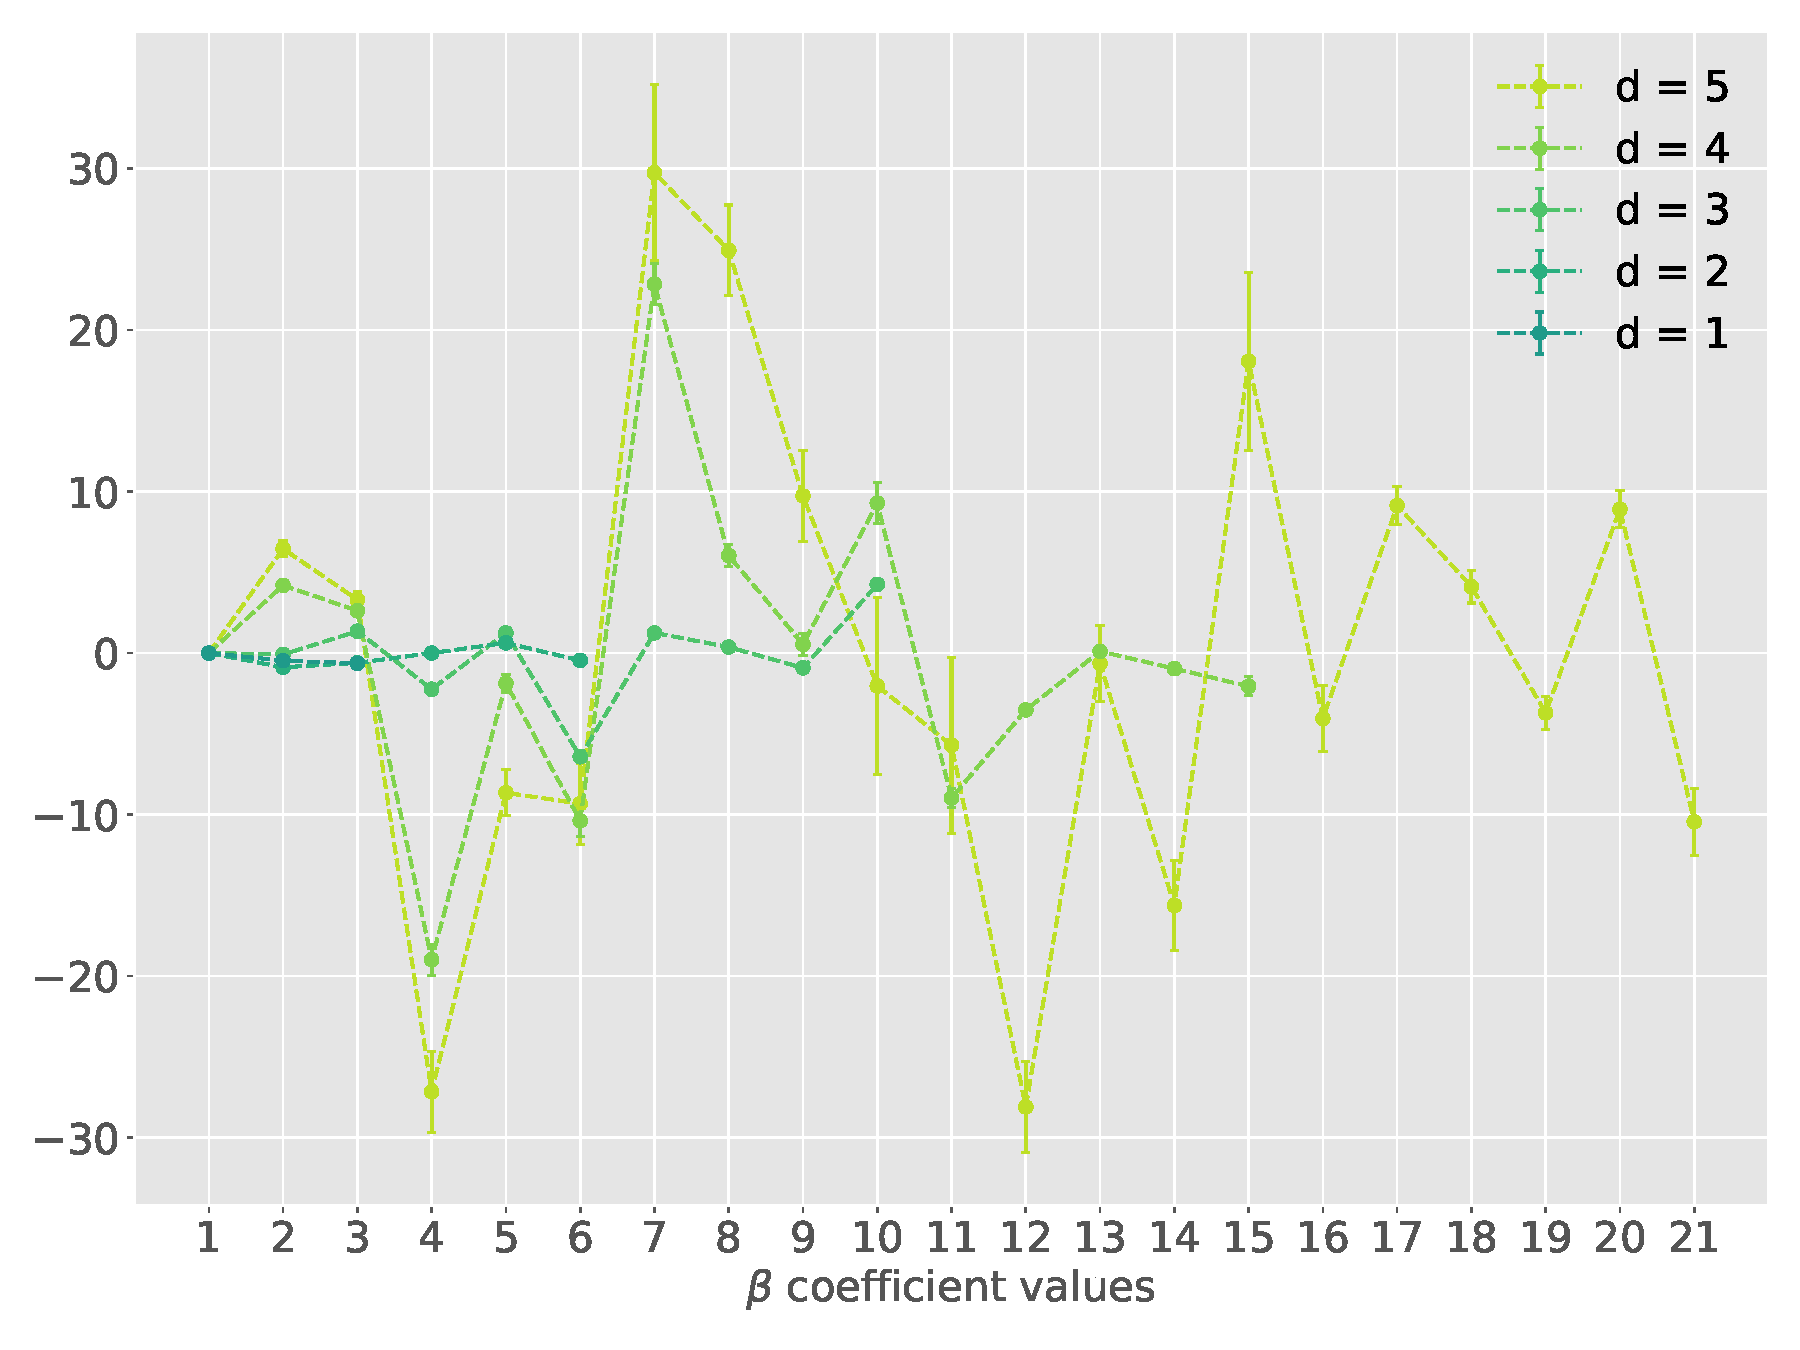
\includegraphics[width=1.0\linewidth]{Project 1/images/OLS_beta.png} %Imports the figure.
    \caption{OLS analysis of the Franke function ($N=XXX, \sigma=XXX$) showing the parameter $\beta$, featuring an error margin of $1\sigma$ XXX,for polynomials up to order $d = 5$.}
    \label{fig: OLS_beta}
\end{figure}

% Not obligatory? 
\begin{figure}[h!]
    \centering %Centers the figure
    \includegraphics[width=1.0\linewidth]{TEMP.jpg} %Imports the figure.
    \caption{OLS analysis of the Franke function presenting the MSE-score for various noise parameters XXX 
    Perhaps include a plot that shows the MSE for train and test data for different noise parameters??? }
    \label{fig: OLS_noise}
\end{figure}


% Part c) Bias-variance trade-off and resampling techniques 
\begin{figure}[h!]
    \centering %Centers the figure
    \includegraphics[width=1.0\linewidth]{TEMP.jpg} %Imports the figure.
    \caption{OLS analysis of the Franke function using a $k = XXX$ bootstrap as a resampling technique.}
    \label{fig: OLS_bootstrap}
\end{figure}

\begin{figure}[h!]
    \centering %Centers the figure
    \includegraphics[width=1.0\linewidth]{TEMP.jpg} %Imports the figure.
    \caption{OLS analysis of the Franke function showing the bias, variance and error XXX for polynomials of order $n=XXX$, generated using a $k=XXX$ bootstrap. }
    \label{fig: OLS_bias-variance}
\end{figure}


% Part d) Cross-validation as resampling techniques 
\begin{figure}[h!]
    \centering %Centers the figure
    \includegraphics[width=1.0\linewidth]{TEMP.jpg} %Imports the figure.
    \caption{OLS analysis of the Franke function using cross-validation with $k = 5-10$ folds as a resampling technique.}
    \label{fig: OLS_crossvalidation}
\end{figure}

% Part e) Ridge Regression on the Franke function with resampling 

% All these show the MSE?? 
\begin{figure}[h!]
    \centering %Centers the figure
    \includegraphics[width=1.0\linewidth]{TEMP.jpg} %Imports the figure.
    \caption{Ridge analysis of the Franke function using a $k = XXX$ bootstrap as a resampling technique.}
    \label{fig: Ridge_bootstrap}
\end{figure}

\begin{figure}[h!]
    \centering %Centers the figure
    \includegraphics[width=1.0\linewidth]{TEMP.jpg} %Imports the figure.
    \caption{Ridge analysis of the Franke function using cross-validation with $k = 5-10$ folds as a resampling technique.}
    \label{fig: Ridge_}
\end{figure}

\begin{figure}[h!]
    \centering %Centers the figure
    \includegraphics[width=1.0\linewidth]{TEMP.jpg} %Imports the figure.
    \caption{Ridge analysis of the Franke function showing the bias, variance and error XXX for polynomials of order $n=XXX$, generated using a $k=XXX$ bootstrap. }
    \label{fig: Ridge_bias-variance}
\end{figure}

% Part f) Lasso Regression on the Franke function with resampling 







Best fit model for the franke function 




% Part g) Analysis of real data 
Plot scaled terrain data representing the part of the map we chose 

1) Plot beta 
OLS
- MSe for train and test data 
- Bias variance 
- heatmap of the prediction MSE as a function of both polynomial degree and penalty parameter lambda 
Ridge: Same as above 

Best fit model for the terrain 












\newpage
%___________________________DISCUSSION___________________________________
\section{Discussion}\label{sec:discussion}
% Regression analysis for the Franke function 


%----------------------------------------------- OLS ------------------------------------------




We begin performing the OLS regression analysis using the invertible matrix method thing 

We do not scale the data, as there is no point in this 

We train models, finding beta hat for polynomials up to 5 
These optimal parameters are plotted in figure ?? 

Include error? sigma_beta = Var(beta hat OLS)^1/2 !! 

THE BETA PLOT: 
As the polynomial degree of the model increase, so does the variation of the parameters 
As the complexity of the model increases -> It wants to hit more points precicely. 
Coefficients of the same features have the same sign for all polynomal degrees -> stable model - we do not want these to change muhc when we use different polynomail degrees for the model 

With optimal parameters for beta hat OLS we can make our predictions by computing the model y tilde = X beta hat OLS on both training and test data. We also compute the MSE and R² score using eqs bla bla , the result of which is shown in fig MSE AND R2 fig!!! 

Describe the image: As the polynomial degree increases we see that MSE decreases while R2 increases. 
What does it mean: The data we attempt to model, in this case the Franke function, is not very well modeled for lower polynomial degrees. 

A LOTOF NOISE WILL LEAD TO THE MSE BEING INNACURATE ALL THE TIME METHINKS 
We include noise of whatever is good for future reference. 

% c) Study the bias-variance trade-off by implementing the bootstrap resampling technique.
% Perform then a bias-variance analysis of the Franke function by studying the MSE value as function of the complexity of your model.
To further inspect the accuracy of the model, we want to test it for higher order polynomials. 
We model higher polynomials?? Should see the MSE increase a lot for the test data 
Train MSE -> The model tries to emaluate the data as best as it can 
Test MSE -> The model fails -> Overfitting. The model is so well fitted to the training data that it can no longer make accurate predictions on the other data. 

We try to make the result more reliable using the bootstrap technique with k = XXX. What is a suitable number of bootstraps and why? 

Bias-Variance tradeoff -> For low order polynomials the error is from the bas, while for higher order the variance. This is where the tradeoff is relevant, the place where the total error switches its dependence from bas to variance is where we find the optimal polynomial -> when p = XXX. 

% d) mplement the k-fold cross-validation algorithm and evaluate again the MSE function resulting from the test folds 
We can also apply cross-validation as a resampling technique, to see the same thing. We use k-fold = XXX 
Here the MSe for the training data degcrease as ecpected. The MSE for the test data reaches a minimum and diverges. Minimum is for p = XXX. 

% Compare the MSE you get from your cross-validation code with the one you got from your bootstrap code. Comment your results. Try 5 − 10 folds 
We investigate the model with p=XXX further, as this is the optimal model for the OLS analysis. ?? If we want ot. 



% Ridge_________________________________________________________
The free parameter is the penalty parameter $\lambda$. 

% e) Perform the same bootstrap analysis as in the part c) (for the same polynomials) cross-validation in part d) but now for different values of λ. 

See how the MSE varies for different penalty parameters $\lambda$ using the same resampling method as we did for the OLS thing. 

Figure: MSe for both the train and test data change as a function of $\lambda$ using 1) bootstrap and 2) cross validatiaon. 
lambda = 0 -> OLS 

% Compare and analyze your results with those obtained in parts b-d). Study the dependence on λ.
Low lambda should be similar to OLS. 
Higher lambda->(same k as beforte) test MSE decreases to a minumum and remains low as lambda increases. We can find the lambda that minimises the test MSE numerically \lambda^\text{Ridge} 

% Study also the bias-variance trade-off as function of various values of the parameter λ. For the bias-variance trade-off, use the bootstrap resampling method. 

Variance remains low for lambda, while the residual error follows the bias. Will reach some minimum at a lambda. (should be similar to the numericall number, as ridge regression is a biased model) 


% Lasso Regression on the Franke function with resampling 
Same analysis for Lasso BUT we perform a grid search on a grid of the MSE values, which are functions of both lambda and p in order to find the optimal lambda and p at the same time (???) 
Next we can plot MSE for the test data predictions. 
Talk about the different models 


Show the best figures for the Franke function and the terrain. 













\newpage
%___________________________DISCUSSION___________________________________
\section{Discussion}\label{sec:discussion}

We began by performing an OLS regression analysis, following the method described in section~\ref{sec: OLS}. 
For the first part, before implementing the bootstrap or cross-validation technique, we did not scale the data EXPLAIN WHY XXX. 





The test MSE can be used to indicate possible regions of low/high bias and variance. 


Approximating a function with a polynomial 
as you increase the order of the polynomial the error of prediction should be lower 
the taylor approximation gets more correct as the order increases 


c is about overfititng MSE for test and train 
if you increase he order of th epolynomial to an amount 
    many points -> high sigma -> points jump 
    the function will try to connect to all points -> not smooth to the middle but tries to reach every point 
    Training: Perfectly fitted -> the more you increase the order the MSE decreases -> at a point your prediction gets worse and worse, as we can see from the test data (the data you want to predict without fitting it) its perfect, but bad predictions -> overfitting -> MSE of test data increases 
    tries to perfectly fit the function (polynomial up to a certain order) 
    
    play with parameters: If you make a higher sigma, the MSE should (overfitting) increase. The order where the test error happans decreases. 
    if you increase the number of points, the order where you get into overfitting increases (enough datapoints-> nothing to worry about) 
    
    nop: check for different number of points at a certain order -> overfitting 
        test mse for different number of points -> error decreases 
        the region of overfitting (test data) gets shifted to the right -> higher orders 
        
        
    Discuss the bias and variance trade-off as function of your model complexity
(the degree of the polynomial) and the number of data points, and possibly also
your training and test data using the bootstrap resampling method.

We can rewrite to bias and variance -> BIAS stays low but MSE increases 
difference between the MSE BIAS var is 0 

d) 
Cross validation -> Recepie -> you have the matrix (select the whole) and shuffle it randomly. I have seven folds and . train and test. for each fold the train and test is different. Selects randomly entries for the train and test data. 

e MSE function resulting from the test folds: Better MSE due to a lower MSE -> due to more datapoints

Compares bootstrap and k-fold : Bootstrap jumps more?? K-fold is smoother 
    K fold should be more stable at a certain order of sigma (2pi) 
    Youre not guaranteed to get certain points in the train data. In cross val every points makes it into both train and test data. You are thus sure that you have included everything in the training. For bootstrap you may miss out on a very important point. 
    
    Week 36 or 28 
    For certain sigma you have more folds and the errors stable up to a higher poluynomial ordwer. 
        Some region of overfitting 

e) Rescaling is important -> destroys beta0 and scales it to lambda (lecture 35 or 36) 
    modify each beta with a lambda 
    
    Plotted MSE for different values of lambda and different orders 
    least error is for very low lambda 
    we shoudl see that there is no point in using Ridge or Lasso as it doesnt decrease the MSE 
    best way is to use the simple, faster model 
    
    BIAS variance tradeoff 
    
Rescaling does not lower the MSE and we dont know why -> Increases the error for the value lambda = 0 -> makes no sense because lambda = 0 means MSE 
    

    




%___________________________CONCLUSION______________________________________
\section{Conclusion}\label{sec:conclusion}
% Present results and error margin 

% We can gain a greater understanding of magnets. We see how we can model complex and large systems 

% We could have obtained even more precise results if we had bla bla bla 

% Further studies may try bla bla bla 




% acknowledgements (optional)
%\begin{acknowledgments} 
%I would like thank myself for writing this beautiful document.
%\end{acknowledgments}

% _________________________________REFERENCES______________________________________
\newpage 
\section*{References}
\printbibliography[heading=none]

\newpage



We find that the variance is 
\begin{align}
    \text{Var}(y_i) 
    & = \mathbb{E}\left\{\left[y_i - \mathbb{E}(y_i)\right]^2\right\} = \mathbb{E}\left(y_i^2\right) - \left[\mathbb{E}\left(y_i^2\right)\right]^2 \nonumber \\ 
    & = \mathbb{E}\left[\left(\mathbf{X}_{i,*}\beta + \varepsilon_i\right)^2\right] - \left(\mathbf{X}_{i,*}\boldsymbol{\beta}\right)^2 \nonumber \\ 
    & = \mathbb{E}\left[\left(\mathbf{X}_{i,*}\boldsymbol{\beta}\right)^2 + 2\varepsilon_i\mathbf{X}_{i,*}\boldsymbol{\beta} + \varepsilon_i^2\right] - \left(\mathbf{X}_{i,*}\boldsymbol{\beta}\right)^2 \nonumber \\ 
    & =(\boldsymbol{X}_{i,*}\boldsymbol{\beta})^2 + 2 \mathbb{E}(\varepsilon_i)\mathbf{X}_{i,*}\boldsymbol{\beta} + \mathbb{E}(\varepsilon^2_i) - (\mathbf{X}_{i,*}\boldsymbol{\beta})^2 \nonumber \\ 
    & = \mathbb{E}(\varepsilon^2_i) = \text{Var}(\varepsilon_i) = \sigma^2, 
\end{align}
hence, $\boldsymbol{y}$ follows a normal distribution with mean value $\mathbf{X}\boldsymbol{\beta}$ and variance $\sigma^2$, that is $y_i\sim N(\mathbf{X}_{i,*}\boldsymbol{\beta},\sigma^2)$. 

With the OLS expressions for the optimal parameters $\boldsymbol{\hat{\beta}}$ we can evaluate the expectation value, 



\begin{align}
    r \equiv \frac{i\Delta t}{2h^2}
\end{align}


%u_{i+1,j}^{n+1} - 2u_{ij}^{n+1} + u_{i-1,j}^{n+1}


\end{document}